\documentclass{beamer}
\mode<presentation>{
  %\setbeamertemplate{background canvas}[vertical
  %shading][bottom=red!10,top=blue!10]

  %\usetheme{Boadilla}
  \usetheme{CambridgeUS}
  \usefonttheme[onlysmall]{structurebold}
}

\setbeamertemplate{enumerate items}[square]
\setbeamertemplate{itemize items}[square]

\usepackage[utf8]{inputenc}
\usepackage{xcolor}
\usepackage{colortbl}
\usepackage{graphicx}


\usepackage{amsmath,amssymb,epsfig}
\usepackage{listings}
\usepackage{multicol}
\usepackage{empheq}
\usepackage{setspace}
\usepackage{hyperref}

% \singlespacing
% nagyon lelogtak avegen a sorok
\linespread{0.6}

\lstset{
  language=matlab,
  numbers=none,
  breaklines=true,
  basicstyle=\small,
  columns=fullflexible,
  %keepspaces=true,
  literate=
  {*}{{\char42}}1
  {-}{{\char45}}1
}

\newcommand{\PC}[1]{\vspace{0.4em} \par\centerline{#1} \vspace{0.4em} }

\definecolor{szurke}{RGB}{210,210,210}
\definecolor{zold}{RGB}{127, 226, 140}
\definecolor{barack}{RGB}{250,240,230}
\definecolor{peldaSz}{RGB}{96, 174, 177}
\definecolor{feladatSz}{RGB}{221, 121, 104}
\definecolor{ismSz}{RGB}{174, 100, 187}
\definecolor{lila}{RGB}{174, 100, 187}
\definecolor{barna}{RGB}{221, 121, 104}
\definecolor{zold2}{RGB}{96, 174, 177} % olyan kekeszold



\newcommand{\code}[1]{\colorbox{szurke}{\texttt{#1}}}
\newcommand{\codeC}[2]{\colorbox{#2}{\texttt{#1}}}

\newcommand*\dobozZold[1]{\colorbox{zold}{\hspace{0.5ex} #1 \hspace{0.5ex} }}
\newcommand*\dobozBarack[1]{\colorbox{barack}{\hspace{1em} #1 \hspace{1em} }}
\newcommand*\sorVerb[1]{\colorbox{barack}{\hspace{0.2em} \texttt{ #1 } \hspace{0.2em} }}
\newcommand*\sorVerbZ[1]{\colorbox{zold}{\hspace{0.2em} \texttt{ #1 } \hspace{0.2em} }}




\newcommand{\kiemelZold}[1]{\begin{empheq}[box=\dobozZold]{gather*} #1 \end{empheq} }


\newcommand{\incFile}[1]{{\lstinputlisting[frame=single,backgroundcolor=\color{barack}]{#1}}}
\newcommand{\incFileC}[2]{{\lstinputlisting[frame=single,backgroundcolor=\color{#2}]{#1}}}

\newcommand{\incFileL}[3]{{\lstinputlisting[firstline=#2,lastline=#3,frame=single,backgroundcolor=\color{barack}]{#1}}}
\newcommand{\incFileLC}[4]{{\lstinputlisting[firstline=#2,lastline=#3,frame=single,backgroundcolor=\color{#4}]{#1}}}


\newcommand{\incCode}[1]{\colorbox{codeColor}{{\lstinline{#1}}}}

\newcommand{\pelda}{\colorbox{peldaSz}{Example}\newline\vskip 0.01em }
\newcommand{\feladat}[1]{{\vskip 1ex}\colorbox{feladatSz}{Exercise #1}\newline}
\newcommand{\solu}[1]{{\vskip 1ex}\colorbox{feladatSz}{Solution #1}\newline}
\newcommand{\tenyek}{\colorbox{zold}{Facts}\newline}
\newcommand{\allitas}{\colorbox{zold2}{Proposition}\newline}
\newcommand{\megj}{\colorbox{zold}{Remark}\newline}
\newcommand{\ism}{\colorbox{ismSz}{Review}\newline}
\newcommand{\zold}[1]{\colorbox{peldaSz}{#1}\newline}
\newcommand{\kek}[1]{\colorbox{ismSz}{#1}\newline}
\newcommand{\kzold}[1]{\colorbox{zold2}{#1}\newline}



\newcommand{\matHigh}[1]{\begin{empheq}[box=\dobozZold]{gather*} #1 \end{empheq} }
\newcommand{\matHighB}[1]{\begin{empheq}[box=\dobozBarack]{gather*} #1 \end{empheq} }



\definecolor{docLinkColor}{RGB}{170,150,230}
\definecolor{linkSz}{RGB}{220,180,140}
\newcommand{\docLink}[2]{\colorbox{linkSz}{\href{#1}{#2}}}
\newcommand{\hint}[1]{{\vskip 0.5ex}\colorbox{linkSz}{\href{run:#1}{Hint}}}
\newcommand{\sol}[1]{{\vskip 0.5ex}\colorbox{zold}{\href{run:#1}{Solution}}}
\newcommand{\data}[1]{{\vskip 0.5ex}\colorbox{linkSz}{\href{run:#1}{The datas in text file}}}
\newcommand{\localLink}[2]{\colorbox{zold}{\href{run:#2}{#1}}}


\author[Noszály Csaba]{NCs}
\date{}


\title{Tanszéki}

\begin{document}

\begin{frame} \maketitle
\end{frame}


\begin{frame}
A dokumentum megtalálható a 
\vspace{0.3cm}
\PC{\url{http://arato.inf.unideb.hu/noszaly.csaba/tanszeki.pdf}}
\vspace{0.3cm}
\par\noindent
helyen.
\end{frame}


\begin{frame}
\begin{figure}%                 use [hb] only if necceccary!
	\centering
	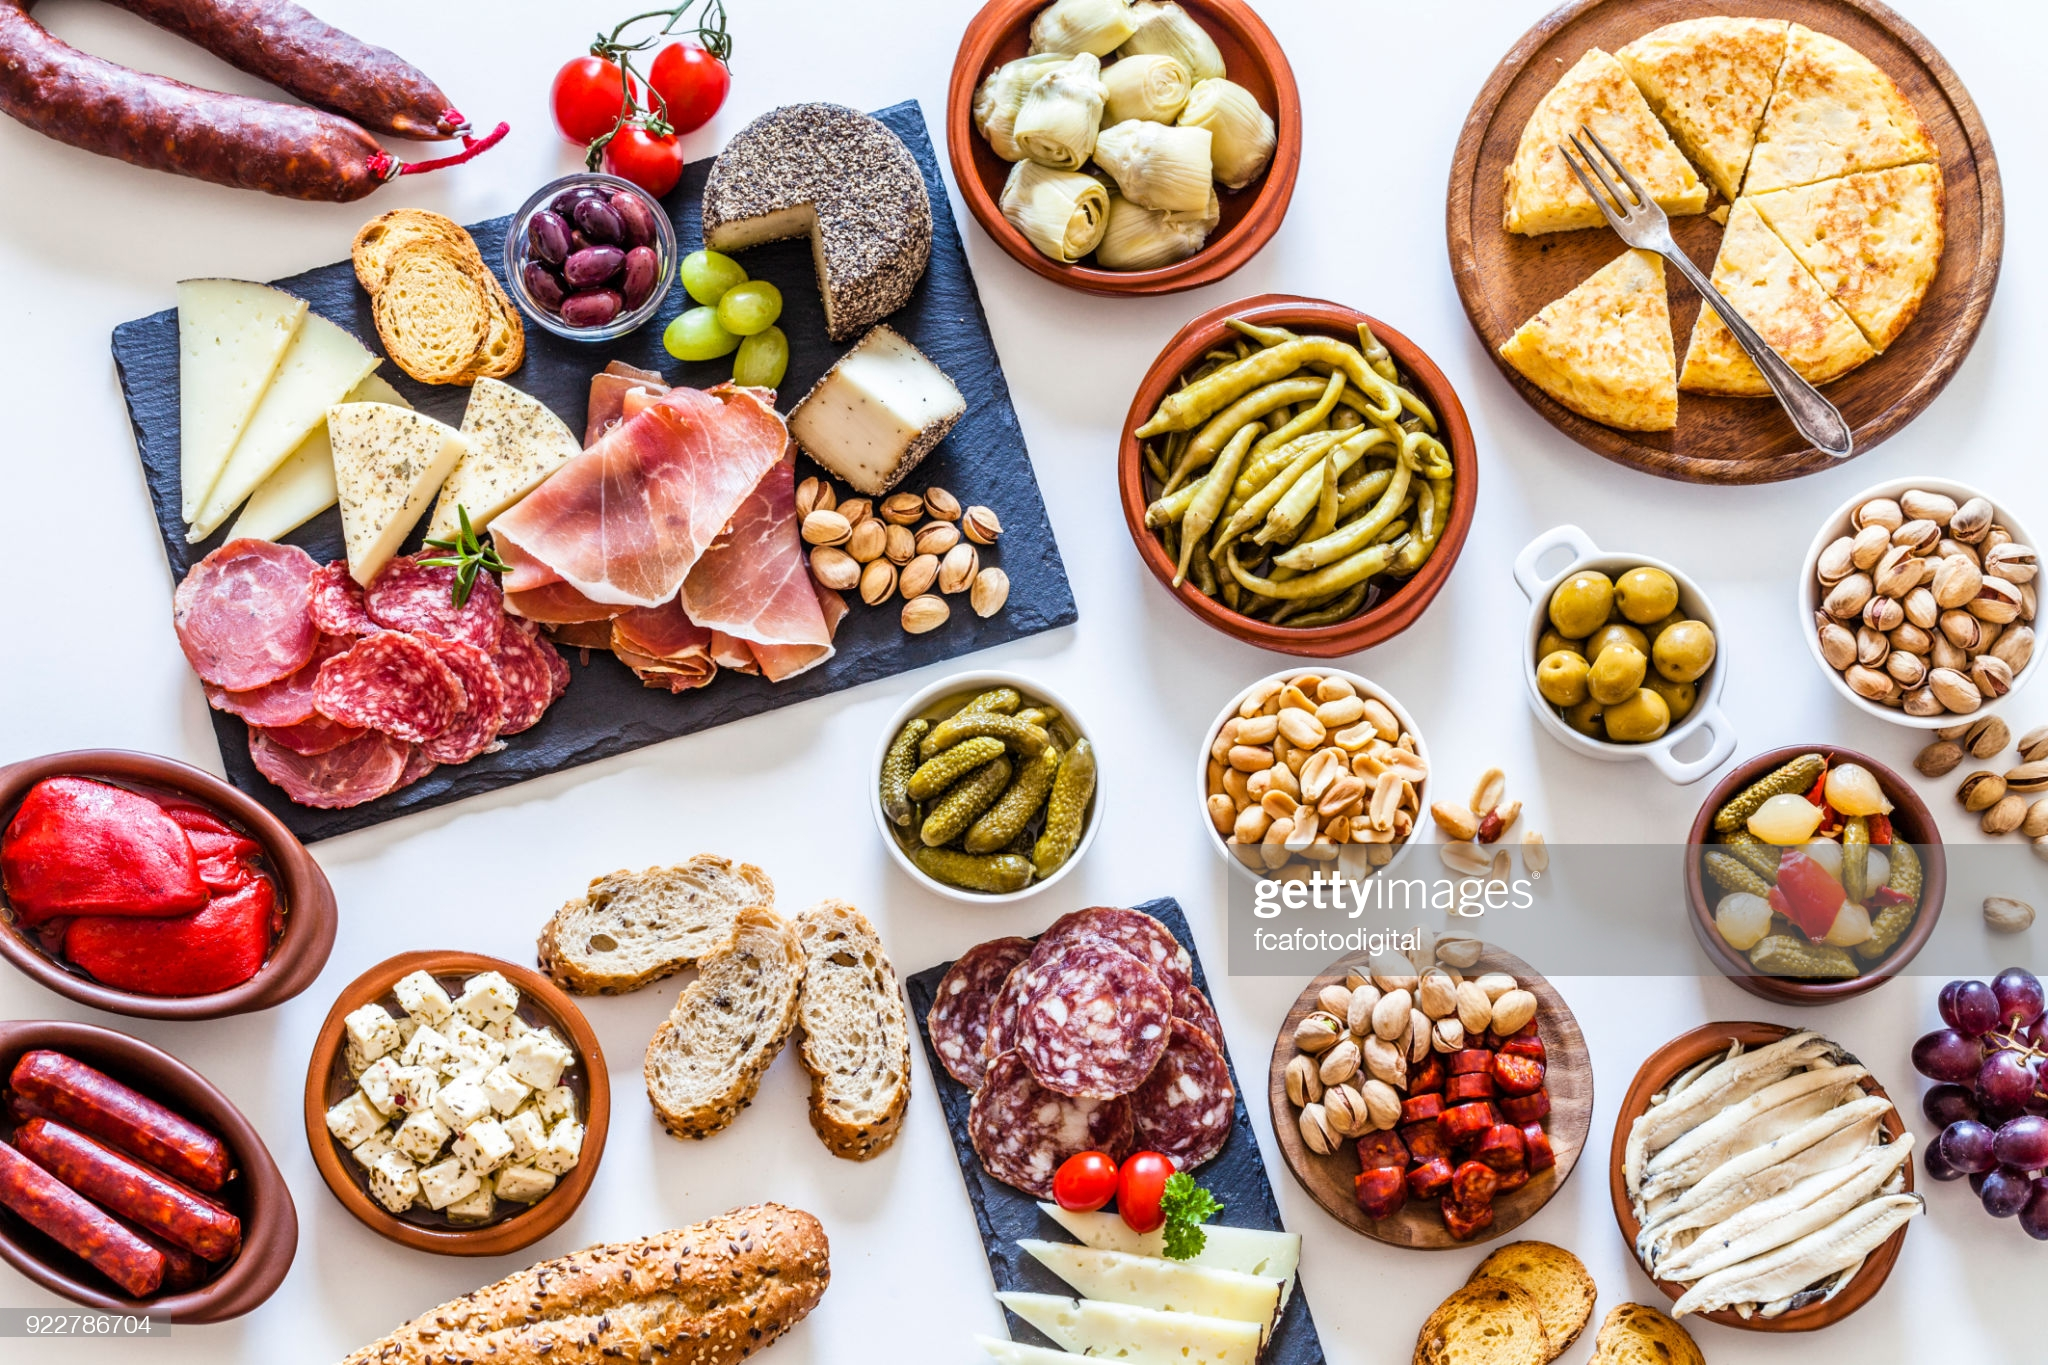
\includegraphics[width=10cm]{tapas.jpg}
	%\caption{tapas}
	\label{fig:tapas}
\end{figure}
\end{frame}




\begin{frame} {Elemi konvergenciatesztek.}

\PC{\dobozZold{A Cauchy-féle $n$. gyök teszt variációja}}\vspace{0.2cm}

\par\noindent Tfh:
\begin{gather*}
a_n\ge 0 \ \ \text{ és } \ \ \frac{\lambda_n}{\log{n}}\to \infty
\end{gather*}
Ekkor:
\begin{gather*}
L<1 \ \implies \ \sum_n a_n< \infty \\
L>1 \ \implies \ \sum_n a_n= \infty
\end{gather*}
ahol
\begin{gather*}
L={\overline{\lim}}_n a_n^{\frac{1}{\lambda_n}}
\end{gather*}

\href{http://bit.ly/3siHgwS}{\dobozBarack{Bővebb leírás}}

\end{frame}


\begin{frame} {Elemi konvergenciatesztek.}

\PC{\dobozZold{A Cauchy-féle $n$. gyök teszt és a Raabe-teszt keverése}}\vspace{0.2cm}

\par\noindent Tfh:
\begin{gather*}
a_n> 0 \ \ \text{ és } \ \ \frac{\lambda_n}{\log{n}}\to \infty
\end{gather*}

Ekkor:
\begin{gather*}
{\underline{\lim}}~ M_n >1 \ \implies \ \sum_n a_n< \infty \\
M_n \le 1 \ \ \text{ elég nagy $n$-re} \ \implies \ \sum_n a_n= \infty
\end{gather*}
ahol
\begin{gather*}
M_n= \frac{\lambda_n}{\log(n)}\left(\frac{1}{a_n^{\frac{1}{\lambda_n}}}-1\right)
\end{gather*}
\href{http://bit.ly/3uR8rQW}{\dobozBarack{Bővebb leírás}}
\end{frame}



\begin{frame} {Elemi konvergenciatesztek.}

\PC{\dobozZold{Cauchy + Raabe V2}}\vspace{0.2cm}

\par\noindent Tfh:
\begin{gather*}
a_n> 0 \ \ \text{ és } \ \ \frac{\lambda_n}{\log{n}}\to \infty
\end{gather*}
Ekkor
\begin{gather*}
{\underline{\lim}}~ N_n >1 \ \implies \ \sum_n a_n< \infty \\
N_n \le 1 \ \ \text{ elég nagy $n$-re} \ \implies \ \sum_n a_n= \infty
\end{gather*}
ahol
\begin{gather*}
N_n= \frac{\lambda_n}{\log(n)}\left( \left(\frac{a_n}{a_{n+1}}\right)^{\frac{1}{\lambda_n}}-1\right)
\end{gather*}


\href{http://arato.inf.unideb.hu/noszaly.csaba/raabevari2.pdf}{\dobozBarack{Bővebb leírás}}
\end{frame}



\begin{frame}
\end{frame}

\end{document}
